\chapter{The plans of the project}
\label{chap:goals}

\section{Definition of my project}

After some interviews with Mr. Champeau, I wrote the table of requirements (Table \ref{tab:requirements}). This table contains all requirements that satisfy the goals of this project define before.

\textit{FS} means service function and \textit{C} means constraints.

\noindent{}
\begin{table}[!h]
  \centering
  \begin{tabular}[h]{|m{0.2\linewidth}|m{0.25\linewidth}|m{0.45\linewidth}|}
    \hline
    \multicolumn{3}{|c|}{Table of requirements}\\
    \hline
    Number&Type of Designation&Designation\\
    \hline
    FS1&UI&Represent the visualization in the UML Model with graphical tools\\
    \hline
    FS2&UML Designer&Works by default with the the Ciprian simulator\\
    \hline
    FS3&Simulator&Have the possibility to change the simulator with other simulator, for example SCCD\\
    \hline
    FS4&Simulation&Give some debugging tools, for example play, stop, \etc...\\
    \hline
    C1&License&Open Source\\
    \hline
    C2&Compatibility&Be multiplatform. Works on Linux, Windows, and Apple.\\
    \hline
    C3&Documentation&Have documentation, code readable, modularity, etc. In that way, this project could be improved during another internship. \\
    \hline
    C4&User&Be user-friendly\\
    \hline
  \end{tabular}
  \caption{Table of requirements}
  \label{tab:requirements}
\end{table}

Then, it is also possible to represent the project with a octopus diagram (Figure \ref{fig:octopus}). This diagram permit to show the interaction of the simulator with the outside world that the client expected.

\begin{figure}[!h]
  \centering
  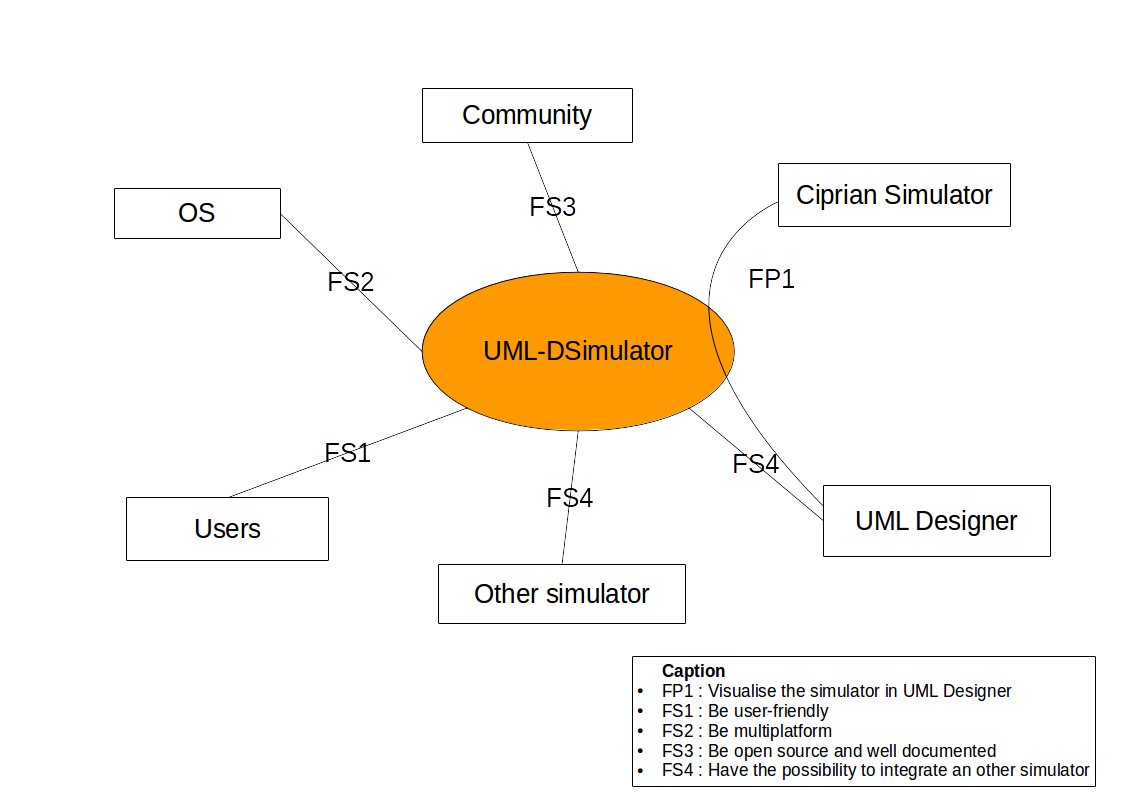
\includegraphics[width=\textwidth]{pieuvre}
  \caption{Octopus diagram}
  \label{fig:octopus}
\end{figure}

\newpage
\section{Goals}

As it was explain in the introduction, the main goal of this project is integrate a simulator in UML Designer. To do that Mr. Ciprian put at my disposal his own Simulator. So it is possible to describe my goals in this order:

\begin{enumerate}
\item Find the way to add plugin in \umld, and understand how it is possible to add more features.
\item Understand how the Ciprian simulator works.
\item Find a way to integrate the simulator but keep the possibility to change it. Moreover it should be kept in mind that the simulator was not finished so the integration of the simulator need to preserve modularity.
\item Propose some debugger tools. For example: a play button, a stop button, \etc.
\item Write documentation and comment in the code to be reusable. Mr Champeau wanted to keep the choice to make some improvements after the end of this internship.
\item Try other simulator and compare its performance with the Ciprian simulator.
\end{enumerate}





% \section{Solution proposed}

% After this definition of the goals and the requirements,

% The main goal of this project is to visualize a simulation of Statechart in UML Designer. The simulator should permit to visualize and debug a model of a state machine. Moreover, UML Designer is a modeling software for UML model and Statechart, so we could create the model and simulate it on the same tools.


% The picture \ref{fig:project} represent the aim of this project.

% \begin{figure}[h]
%   \centering
%   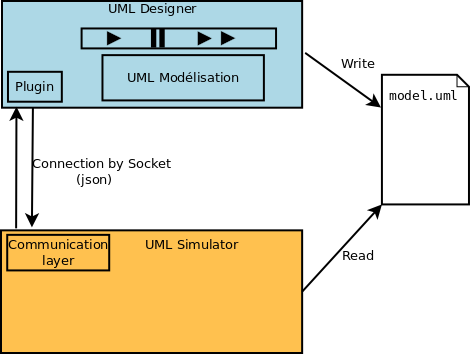
\includegraphics[width=\textwidth]{project}
%   \caption{Description of the project}
%   \label{fig:project}
% \end{figure}







\section{Tools at my disposal}

This section presents a short description of \umld and the Ciprian Simulator. More details can be found in the appendix \ref{chap:UMLDesigner} and \ref{chap:simulator}.
\newpage
\subsection{\umld}
\begin{figure}[!h]
  \begin{minipage}[h]{0.45\linewidth}
    \centering
    
\includegraphics[width=0.6\textwidth]{logo}
    \caption{UML Designer logo}
    \label{fig:logo}
  \end{minipage}\hfill
  \begin{minipage}[h]{0.45\linewidth}

    At the beginning of this project, some tools were at my disposal. First of all, it was \umld created by the french company \textit{Obeo}. It is an open source software documented so I could download the source and work on it. It is a UML modeler with a user interface. It is based on Eclipse and Sirius. It follows the UML2 standard which is well known and documented.

  \end{minipage}
\end{figure}


\subsection{Simulator}
\begin{figure}[!h]
  \begin{minipage}[h]{0.45\linewidth}

    Then, Mr Ciprian Teodorov, one of my professors, has developed a simulator for UML Model. This simulator needed some improvements, but it was a good starting point for this project.

  \end{minipage}\hfill
  \begin{minipage}[h]{0.45\linewidth}
    \centering
    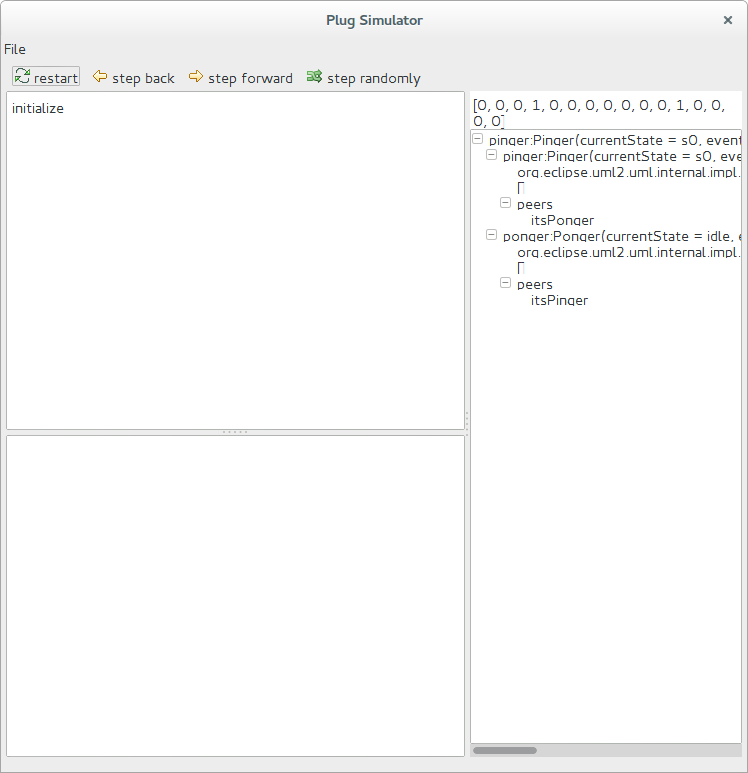
\includegraphics[width=0.9\textwidth]{simulator}
    \caption{Mr Teodorov simulator}
    \label{fig:sim}
  \end{minipage}
\end{figure}







%%% Local Variables:
%%% mode: latex
%%% TeX-master: "../rapport_de_base"
%%% End:
